\chapter{Естественный способ задания движения. Определение скорости и ускорения
точки. Нормальное, касательное ускорения. Их физический смысл. Определение
касательного и нормального ускорений при координатном способе задания движения.}

Естественный способ задания движения применяется в случае, когда траектория
точки заранее известна. Выберем на траектории неподвижную точку \( O \), которую
назовём началом отсчёта дуговой координаты. Положение движущейся точки \( M \)
на траектории будем определять дуговой координатой, то есть расстоянием
\( OM = s \) вдоль траектории.

Расстояния, отложенные в одну сторону от \( O \) будем считать положительными, а
в противоположную -- отрицательными, то есть установим направление отсчёта
дуговой координаты.

Тогда при движении точки \( M \) имеет место соотношение \( s = f(t) \),
называемое уравнением движения точки.

\section{Скорость}

\begin{table}[h!]
    \begin{tabular}{C{.4}m{.55\textwidth}}
        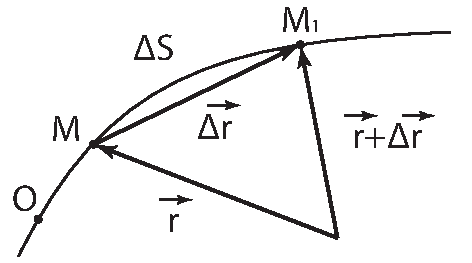
\includegraphics[width=.4\textwidth]{06_velocity} &
        Проведем в точку радиус-вектор \( \vec{r} \). Тогда, по определению:
        \[
            \vec{v} = \der{\vec{r}}{t} = \der{\vec{r}}{s}\cdot\der{s}{t}.
        \]

        Рассмотрим вектор \( \ds \der{\vec{r}}{s} \). Он направлен по
        касательной к траектории и имеет единичную длину,
    \end{tabular}
\end{table}

так как \( \ds \left|\der{\vec{r}}{s}\right| = \lim_{M\to M'}\frac{MM'}
{\smallsmile MM'} = 1 \). То есть \( \ds\der{\vec{r}}{s} \) является ортом
направления касательной и направлен в сторону увеличения дуговой координаты:
\( \ds \vec{\tau} = \der{\vec{r}}{s} \).

Таким образом, \( \ds \vec{v} = \vec{\tau}\cdot\der{s}{t} \). Производная
\( \ds \der{s}{t} \) есть проекция скорости \( \vec{v} \) на касательную, то
есть определяет алгебраическую величину скорости: \( \ds \tilde{v} =
\der{s}{t} \), а её модуль \( \ds v = |\tilde{v}| = \left|\der{s}{t}\right| \).

\section{Ускорение}

По определению ускорение: \( \ds \vec{a} = \der{\vec{v}}{t} \):
\( \ds
    \vec{a} = \der{}{t}\left(\vec{\tau}\cdot\der{s}{t}\right) = \der{\tau}{t}
    \cdot\der{s}{t} + \vec{\tau}\cdot\dder{s}{t}.
\)

Вектор \( \ds \der{\vec{\tau}}{t} = \der{\vec{\tau}}{s}\cdot\der{s}{t} \). Из
дифференциальной геометрии \( \ds \der{\vec{\tau}}{s} = \vec{k} =
\vec{n}\cdot\frac{1}{\rho} \), где \( \rho \) -- радиус кривизны,
\( \vec{k} \) -- кривизна. Следовательно,
\[
    \vec{a} = \vec{n}\cdot\frac{\left(\der{s}{t}\right)^2}{\rho} + \vec{\tau}
    \cdot\dder{s}{t} = \vec{n}\cdot\frac{v^2}{\rho}+ \vec{\tau}\cdot\dder{s}{t}.
\]
Первое слагаемое называется нормальным ускорением, второе -- касательным:
\[
    \vec{a}_n = \vec{n}\cdot\frac{v^2}{\rho}, \quad \vec{a}_\tau =
    \vec{\tau}\cdot\dder{s}{t} = \vec{\tau}\cdot\dder{\tilde{v}}{t}.
\]

Таким образом, проекция ускорения точки на нормаль всегда положительна, а
нормальное ускорение направлено к центру кривизны траектории в данной точке.
Проекция ускорения на касательную равна второй производной от дуговой координаты
по времени. Так как эти две компоненты ускорения взаимно перпендикулярны, то для
модуля полного ускорения имеем \( a = \sqrt{a_n^2 + a_\tau^2} \).

Также вводя алгебраическую величину касательного ускорения, получим
\( \ds \tilde{a}_\tau = \der{\tilde{v}}{t} = \dder{s}{t} \),
\( \ds a_\tau = |\tilde{a}_\tau| = \left|\dder{s}{t}\right| \).

При координатном способе можно определить непосредственным дифференцированием
полное и касательное ускорения: \( \vec{a} = \bigl\{ \ddot{x}, \ddot{y},
\ddot{z}\bigr\} \),
\[
    \vec{a}_\tau = \frac{(\vec{a}\cdot\vec{v})\cdot\vec{v}}{v^2} = \frac{(
    \dot{x}\ddot{x} + \dot{y}\ddot{y} + \dot{z}\ddot{z})}{\dot{x}^2 + \dot{y}^2
    + \dot{z}^2}\cdot\bigl\{\dot{x}, \dot{y}, \dot{z}\bigr\},
\]
а нормальное ускорение может быть найдено из выражения \( \vec{a} = \vec{a}_\tau
+ \vec{a}_n \): \( \vec{a}_n = \vec{a} - \vec{a}_\tau \).

\newpage
